\chapter{Distribution of CH$_{3}$NH$_{2}$ lines contaminated by other molecular line emission in Orion-KL
\label{chap:appendixB}}

\section{Integrated intensity maps}
Out of 24 selected transitions in our observational frequency range, 16 CH$_{3}$NH$_{2}$ transitions are 
blended or masked by other spectral features, or its signal are below the noise level.

In Appendix B, we list 16 transitions that we could not detect.
\newpage

\renewcommand{\arraystretch}{1.5}
\begin{table}[H]
\begin{center}

  \caption{Summary of transition}
  \label{tab:blendOri}
{\scriptsize
  \begin{tabular}{cccccl} \hline
   Fequency [GHz]& S$\mu ^{2}$ [D$^2$] & E$_{\rm{u}}$ [K]& Transition ($J$, $K_{\rm{a}}$, $\Gamma$) & Noise [K]  &Comments \\ \hline 
222.846&  117.24&  156.55&  11, 2, $B_{1}$ $\rightarrow$ 11, 1, $B_{2}$    &  0.084&  SV data \\
227.545&  105.11&  133.16&  10, 2, $B_{2}$ $\rightarrow$ 10, 1, $B_{1}$    &  0.351&  SV data\\
231.844&  93.40&  111.90&  9, 2, $B_{1}$ $\rightarrow$ 9, 1, $B_{2}$   &  0.462&  SV data\\
242.625&  56.31&  399.37&  18, 3, $B_{2}$ $\rightarrow$ 17, 4, $B_{1}$   &  0.534& SV data  \\
231.524&  55.71&  399.38& 18, 3, $E_{1-1}$ $\rightarrow$ 17, 4, $E_{1-1}$  &  0.035&  Reported in Pagani+17\\
218.221&  50.47&  59.97& 7, 0, $E_{1+1}$ $\rightarrow$ 6, 1, $E_{1+1}$  &  3.639&  \\
219.151&  42.23&  92.22& 8, 2, $E_{1-1}$ $\rightarrow$ 8, 1, $E_{1+1}$  &  0.065&  \\
227.997&  39.83&  92.64&  8, 2, $E_{1+1}$ $\rightarrow$ 8, 1, $E_{1+1}$   &  0.118&  SV data\\
231.061&  38.44&  75.61&  7, 2, $E_{1+1}$ $\rightarrow$ 7, 1, $E_{1+1}$  &  1.057&  \\
233.802&  35.87&  60.71&  6, 2, $E_{1+1}$ $\rightarrow$ 6, 1, $E_{1+1}$   &  0.024&  \\
231.576&  35.30&  239.73&  14, 2, $E_{1+1}$ $\rightarrow$ 13, 3, $E_{1+1}$  &  0.033&  Reported in Pagani+17\\
216.843&  34.42&  132.81&  10, 2, $E_{2+1}$ $\rightarrow$ 10, 1, $E_{2+1}$  &  0.074&  \\
251.128&  33.32&  92.22& 8, 2, $E_{1-1}$ $\rightarrow$ 8, 1, $E_{1-1}$ &  0.153&  \\
218.409&  32.65&  17.30&  3, 1, $E_{1+1}$ $\rightarrow$ 2, 0, $E_{1+1}$  &  0.059&  \\
217.6701&  32.53&  156.54& 11, 2, $E_{1+1}$ $\rightarrow$ 11, 1, $E_{1+1}$ &  0.033&  Reported in Pagani+17 \\
237.143&  14.76&  21.99& 2, 2, $E_{1-1}$ $\rightarrow$ 2, 1, $E_{1-1}$ &  0.048&  Reported in Pagani+17 \\ \hline
  \end{tabular}
  }
\end{center}
\end{table}


\newpage

%%%%% 積分強度図挿入 %%%%%
\begin{figure}[H] 
\begin{center}

%%%% ここから
\begin{minipage}{0.98\textwidth} 
\begin{center}
\begin{minipage}{0.48\textwidth}
\begin{center}
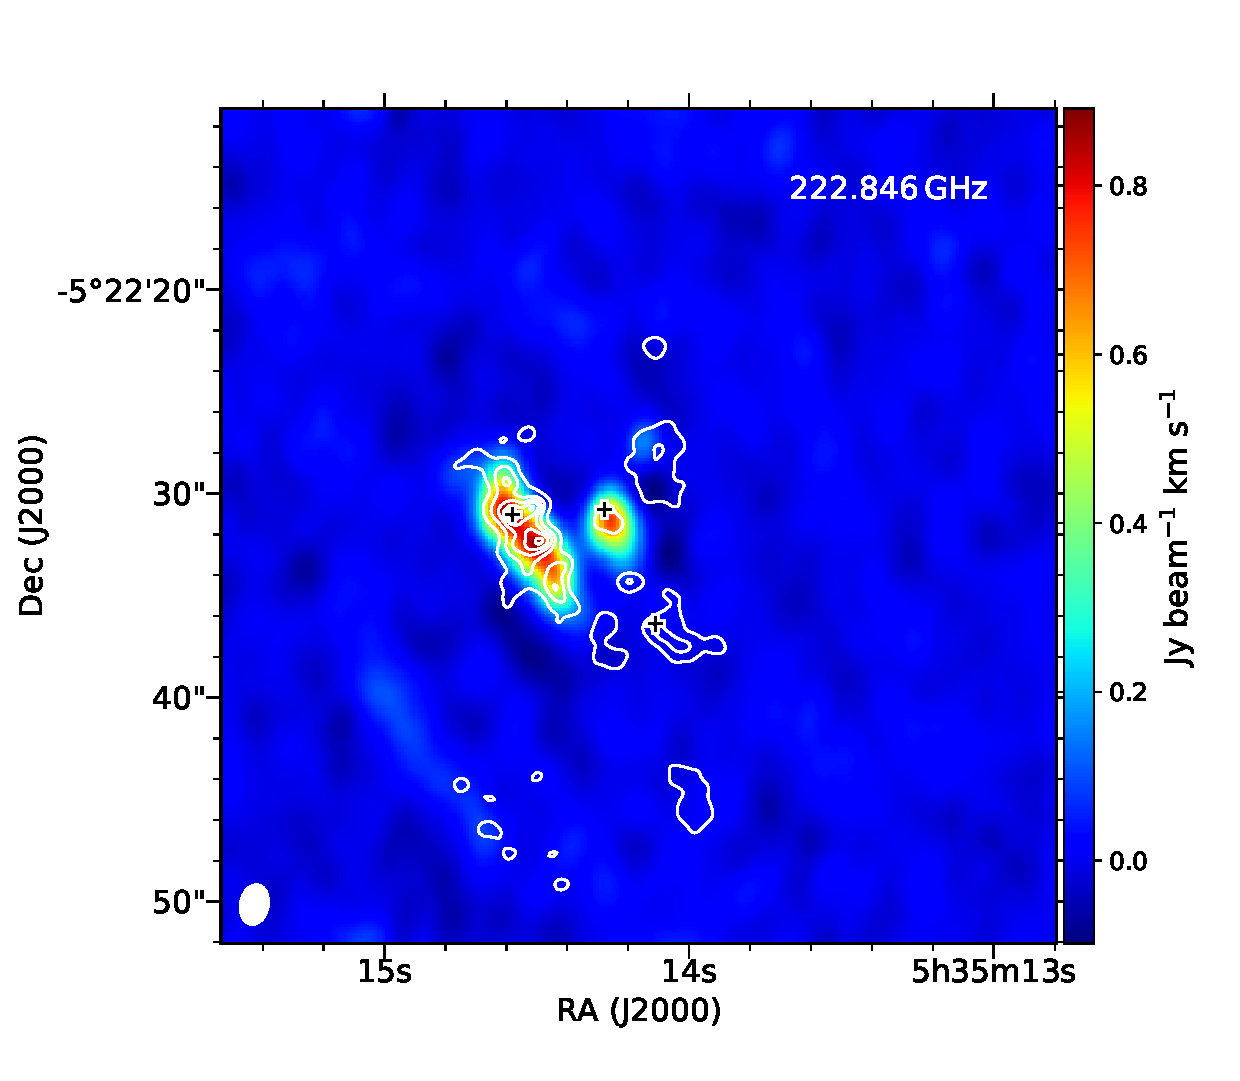
\includegraphics[width=0.98\textwidth]{OrionKL/mom0/222.846SV_mom0_3-7.eps}
%\\(a) 左の図の説明
\end{center}
\end{minipage}
\begin{minipage}{0.48\textwidth}
\begin{center}
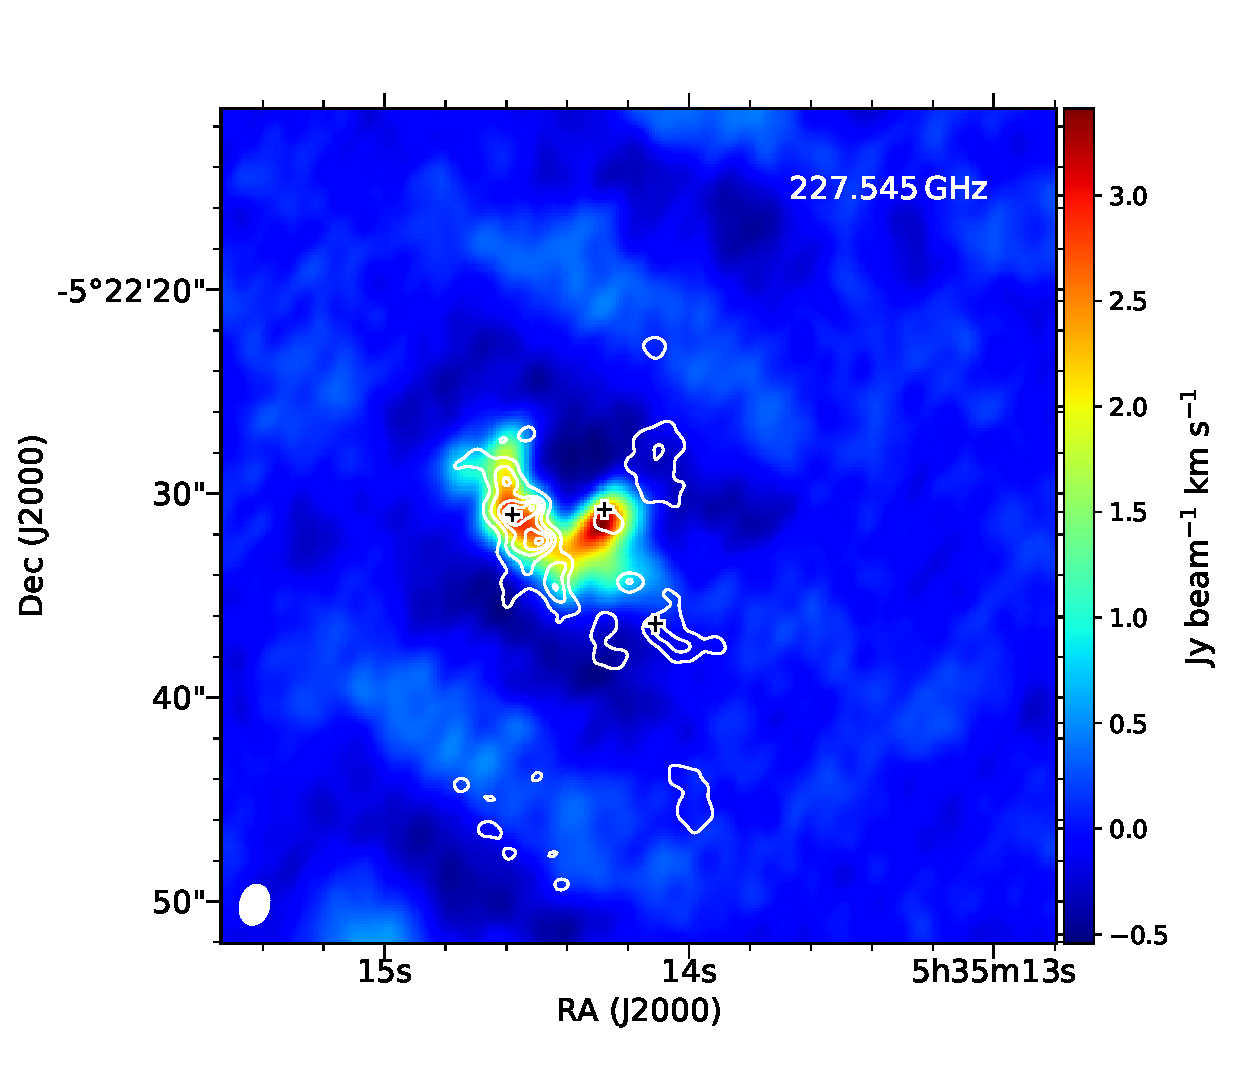
\includegraphics[width=0.98\textwidth]{OrionKL/mom0/227.545SV_mom0_3-7.eps}
%\\(b) 右の図の説明
\end{center}
\end{minipage}
\end{center}
\end{minipage}
%%%% ここまで一組
%%%% ここから
\begin{minipage}{0.98\textwidth} 
\begin{center}
\begin{minipage}{0.48\textwidth}
\begin{center}
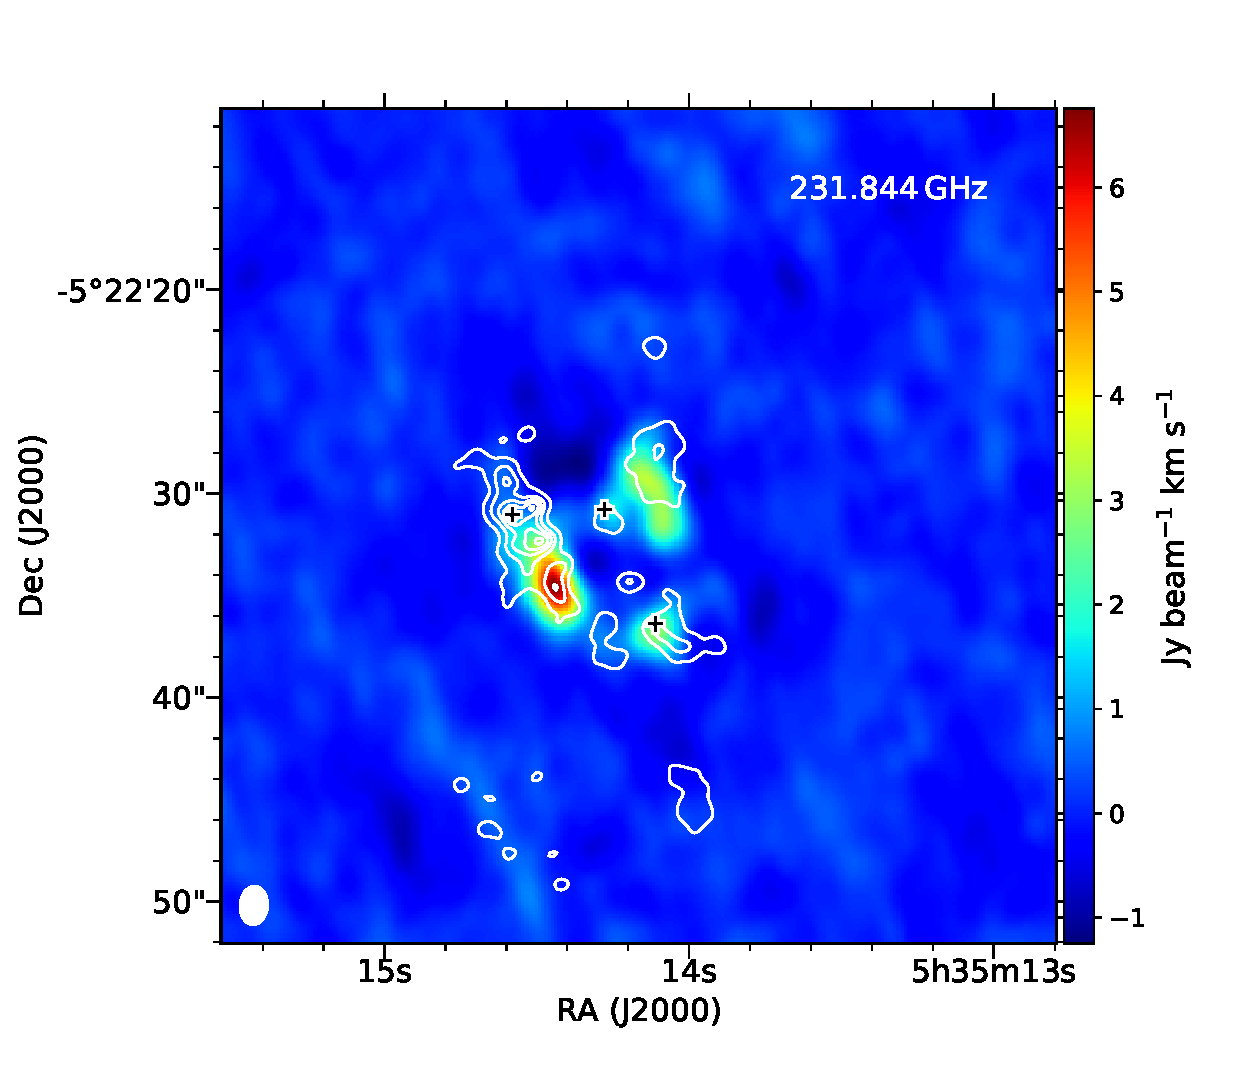
\includegraphics[width=0.98\textwidth]{OrionKL/mom0/231.844SV_mom0_3-7.eps}
%\\(c) 左の図の説明
\end{center}
\end{minipage}
\begin{minipage}{0.48\textwidth}
\begin{center}
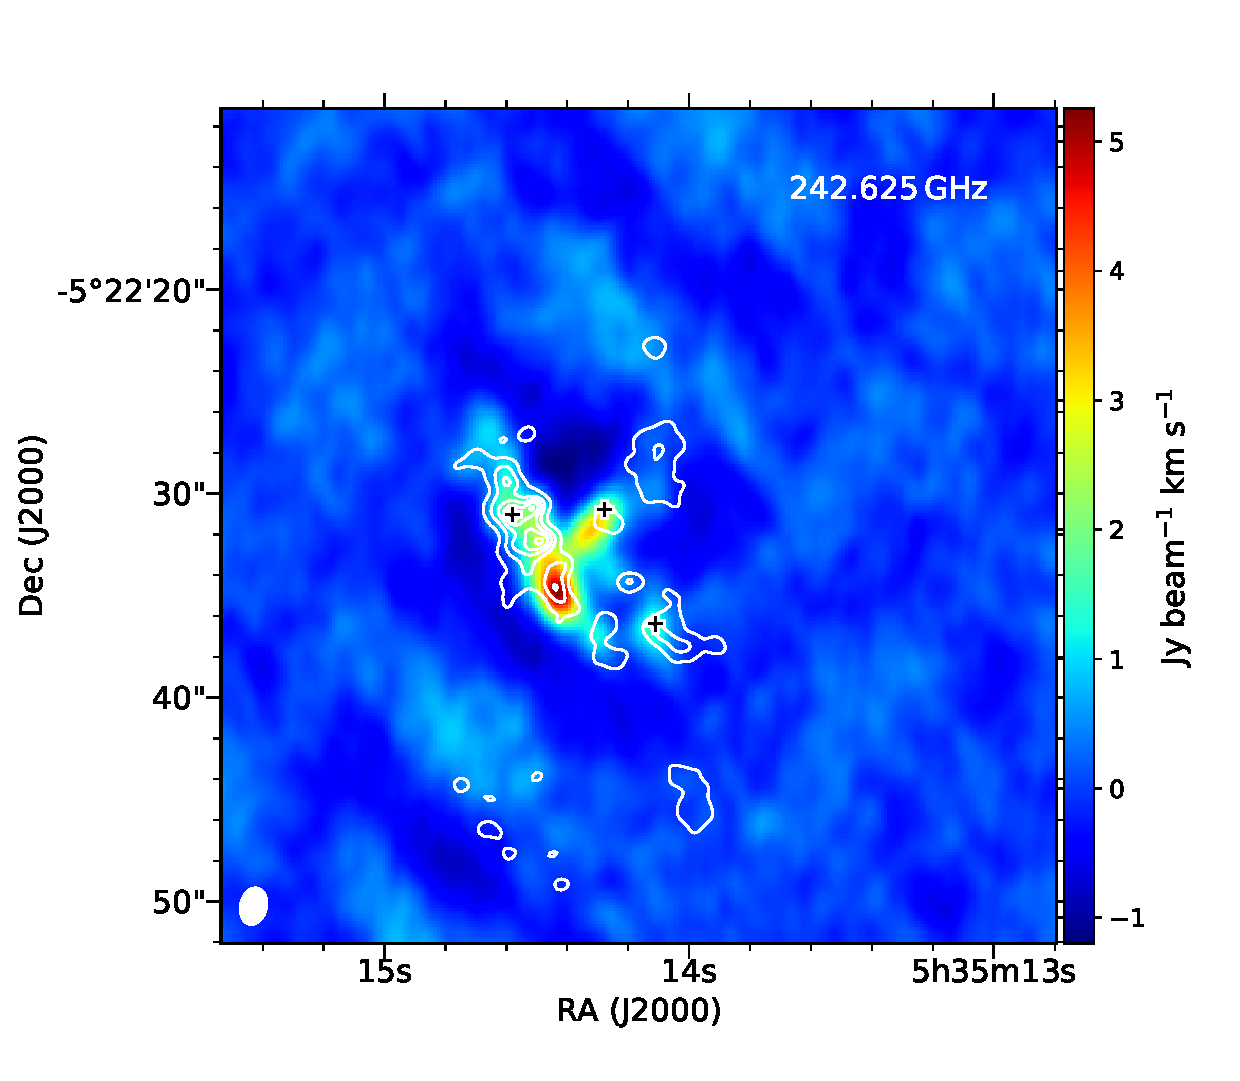
\includegraphics[width=0.98\textwidth]{OrionKL/mom0/242.625SV_mom0_3-7.eps}
%\\(d) 右の図の説明
\end{center}
\end{minipage}
\end{center}
\end{minipage}

\begin{minipage}{0.98\textwidth} 
\begin{center}
\begin{minipage}{0.48\textwidth}
\begin{center}
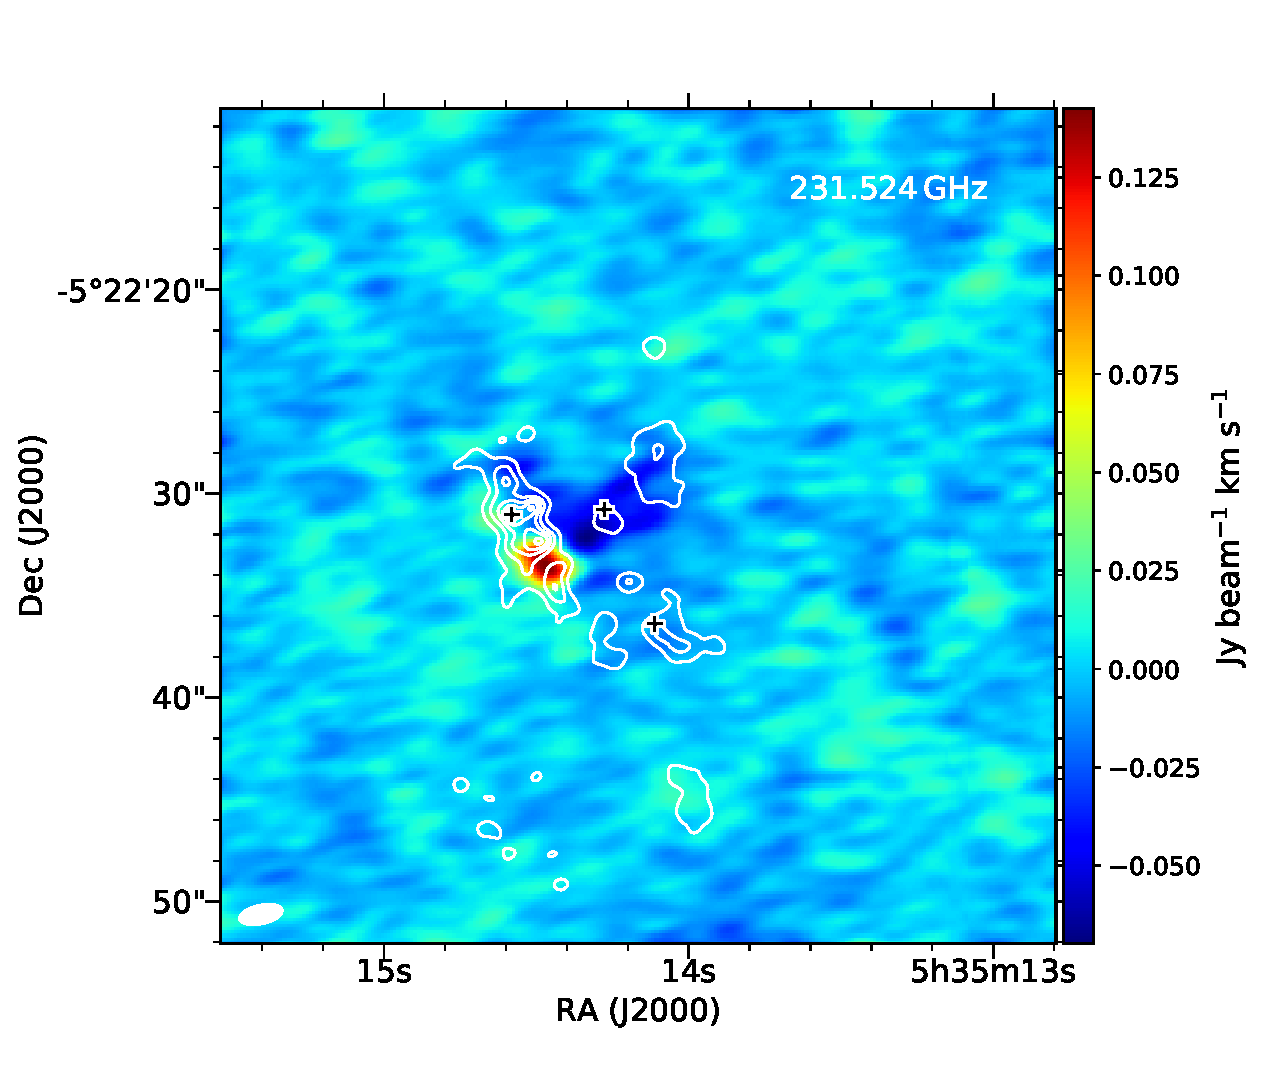
\includegraphics[width=0.98\textwidth]{OrionKL/mom0/231.524mom0_3-7.eps}
%\\(a) 左の図の説明
\end{center}
\end{minipage}
\begin{minipage}{0.48\textwidth}
\begin{center}
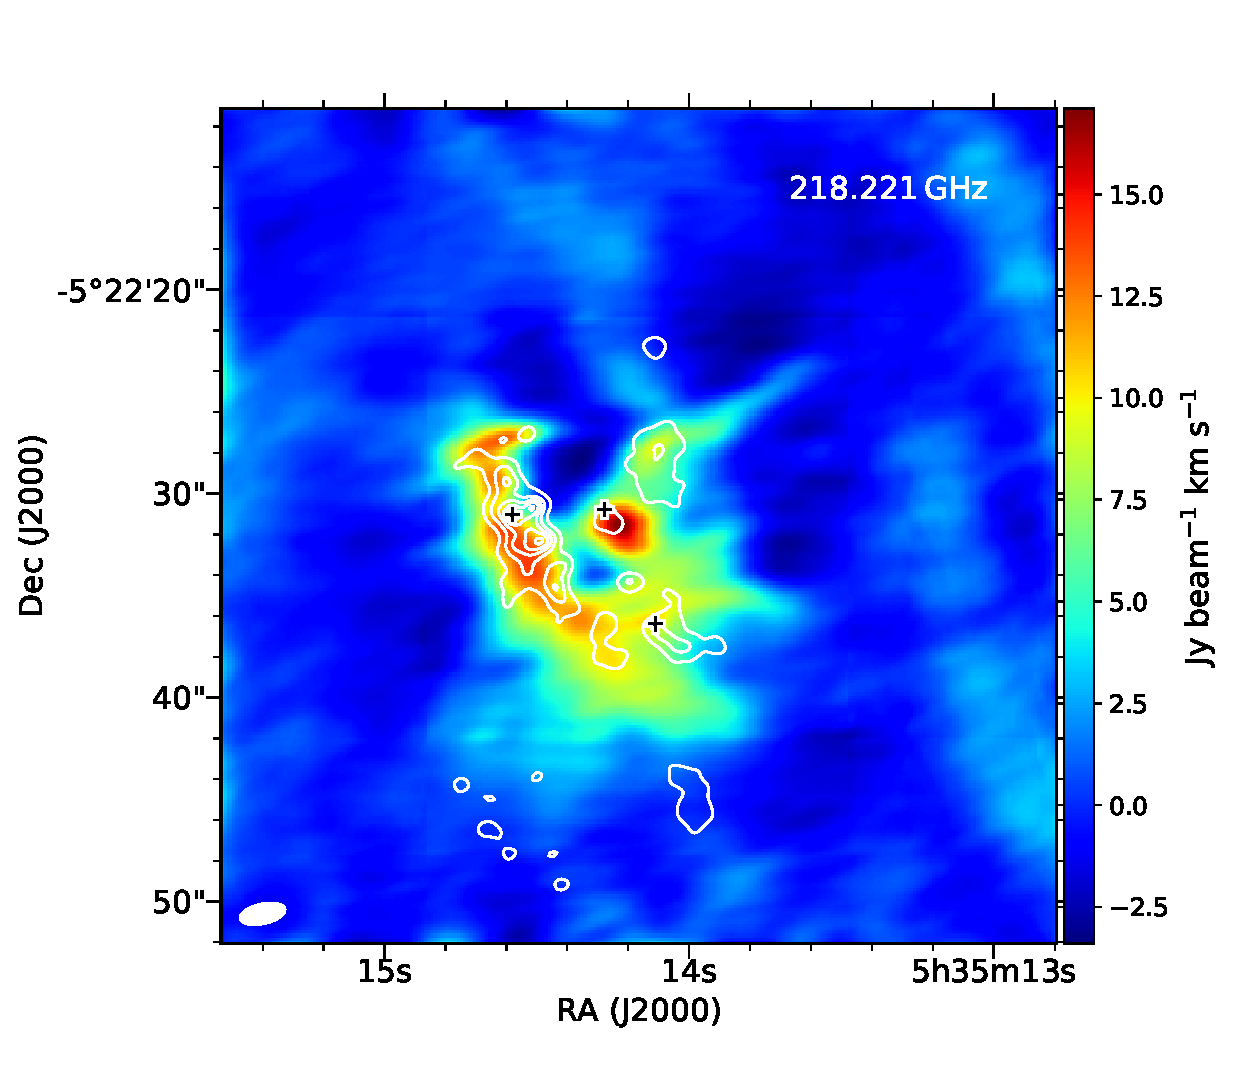
\includegraphics[width=0.98\textwidth]{OrionKL/mom0/218.221mom0_3-7.eps}
%\\(b) 右の図の説明
\end{center}
\end{minipage}
\end{center}
\end{minipage}
%%%% ここまで一組
\caption{Integrated intensity maps around CH$_{3}$NH$_{2}$ line.}
\end{center}
\end{figure}
%%%%%% ここまで

\newpage

%%%%% 積分強度図挿入 %%%%%
\begin{figure}[H] 
\begin{center}
\begin{minipage}{0.98\textwidth} 
\begin{center}
\begin{minipage}{0.48\textwidth}
\begin{center}
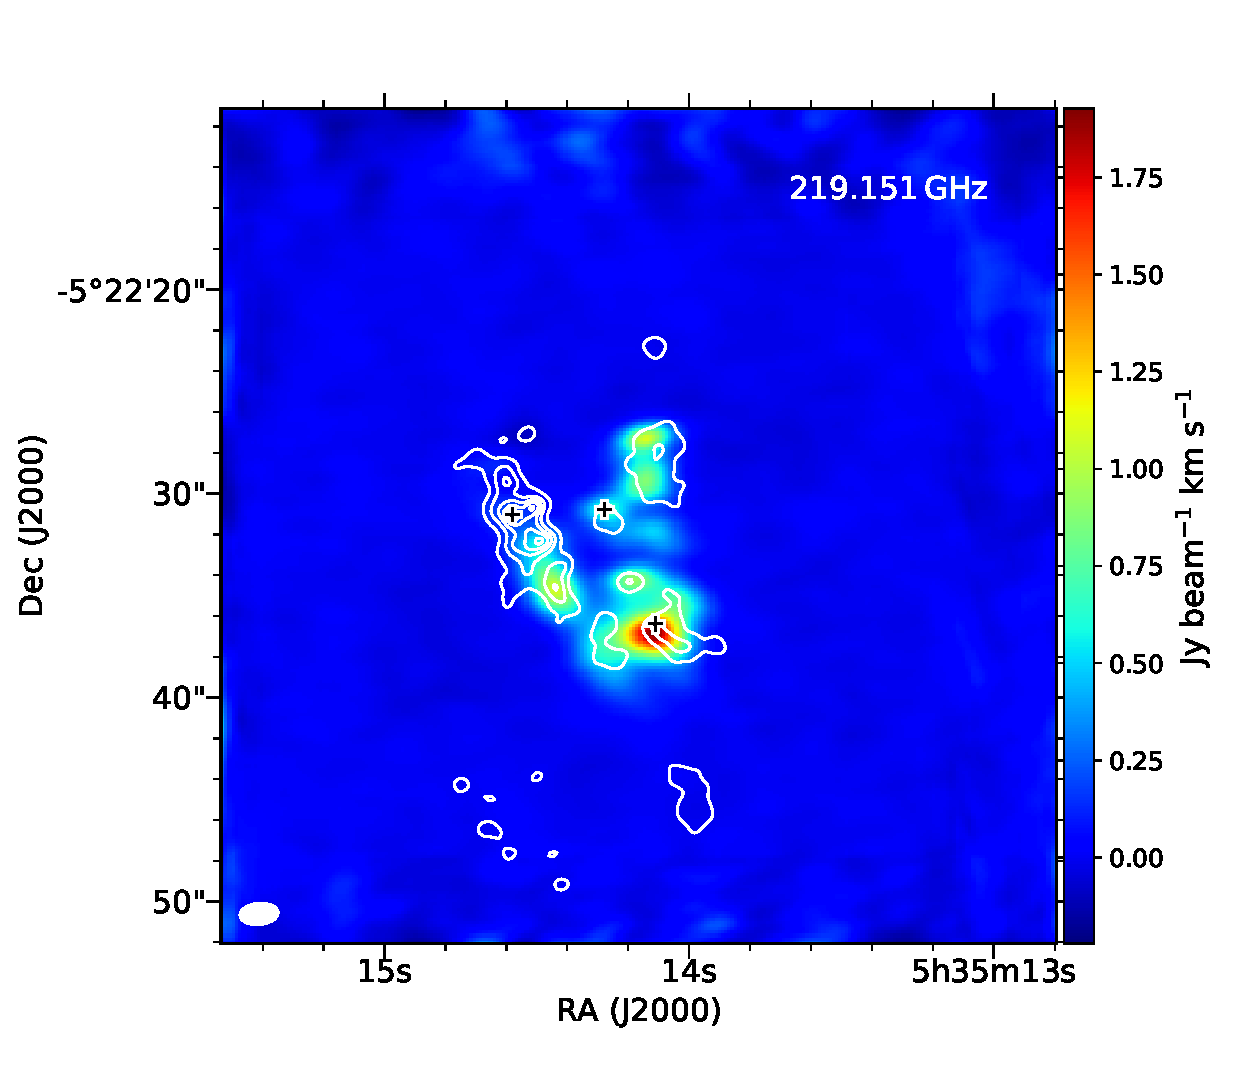
\includegraphics[width=0.98\textwidth]{OrionKL/mom0/219.151mom0_3-7.eps}
%\\(c) 左の図の説明
\end{center}
\end{minipage}
\begin{minipage}{0.48\textwidth}
\begin{center}
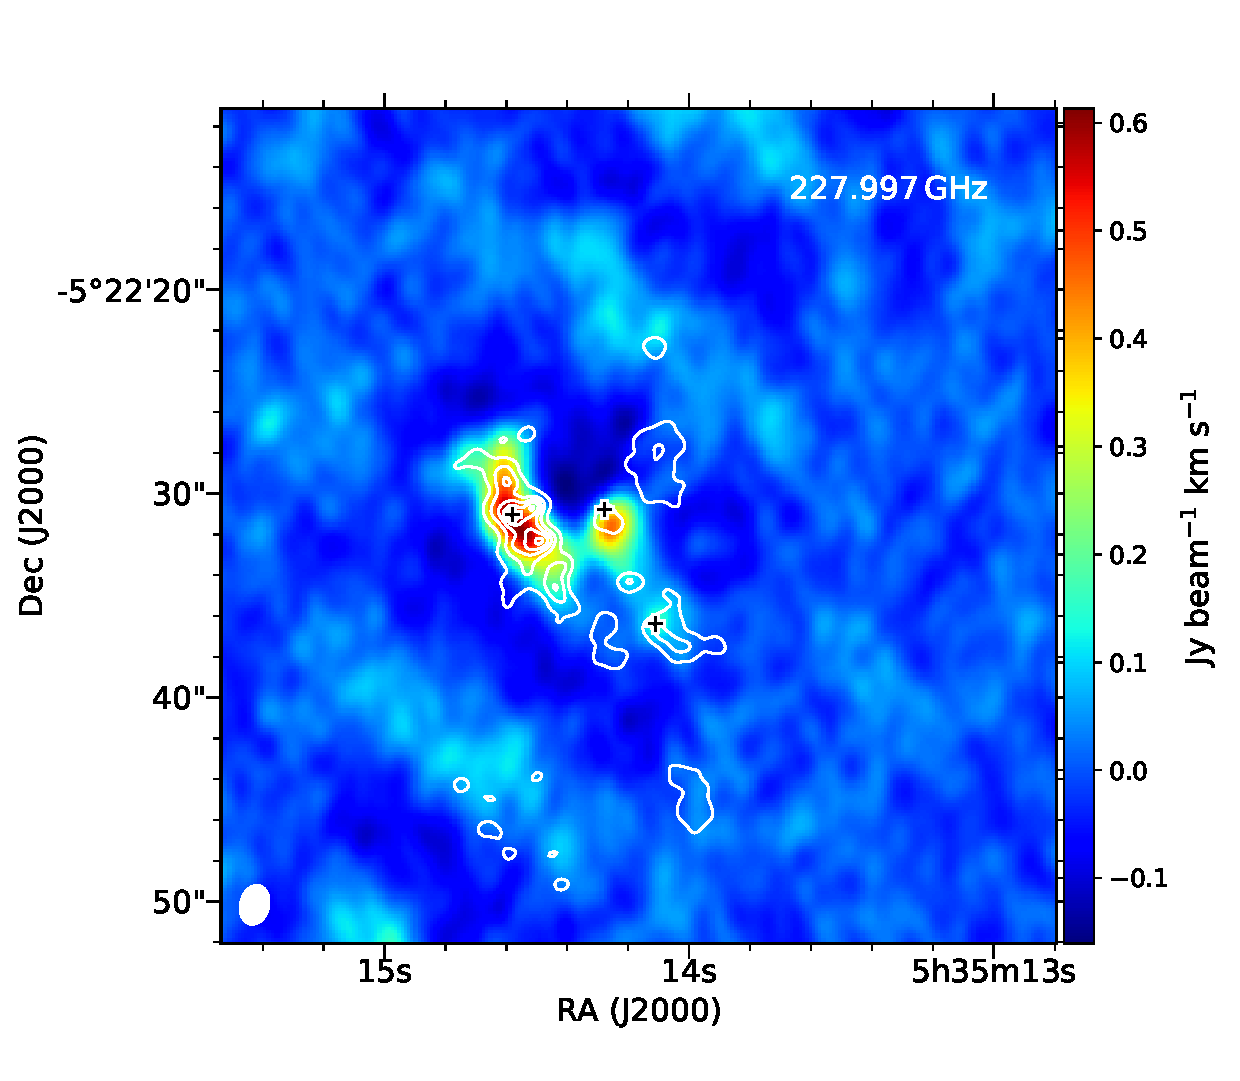
\includegraphics[width=0.98\textwidth]{OrionKL/mom0/227.997SV_mom0_3-7.eps}
%\\(d) 右の図の説明
\end{center}
\end{minipage}
\end{center}
\end{minipage}

%%%% ここから
\begin{minipage}{0.98\textwidth} 
\begin{center}
\begin{minipage}{0.48\textwidth}
\begin{center}
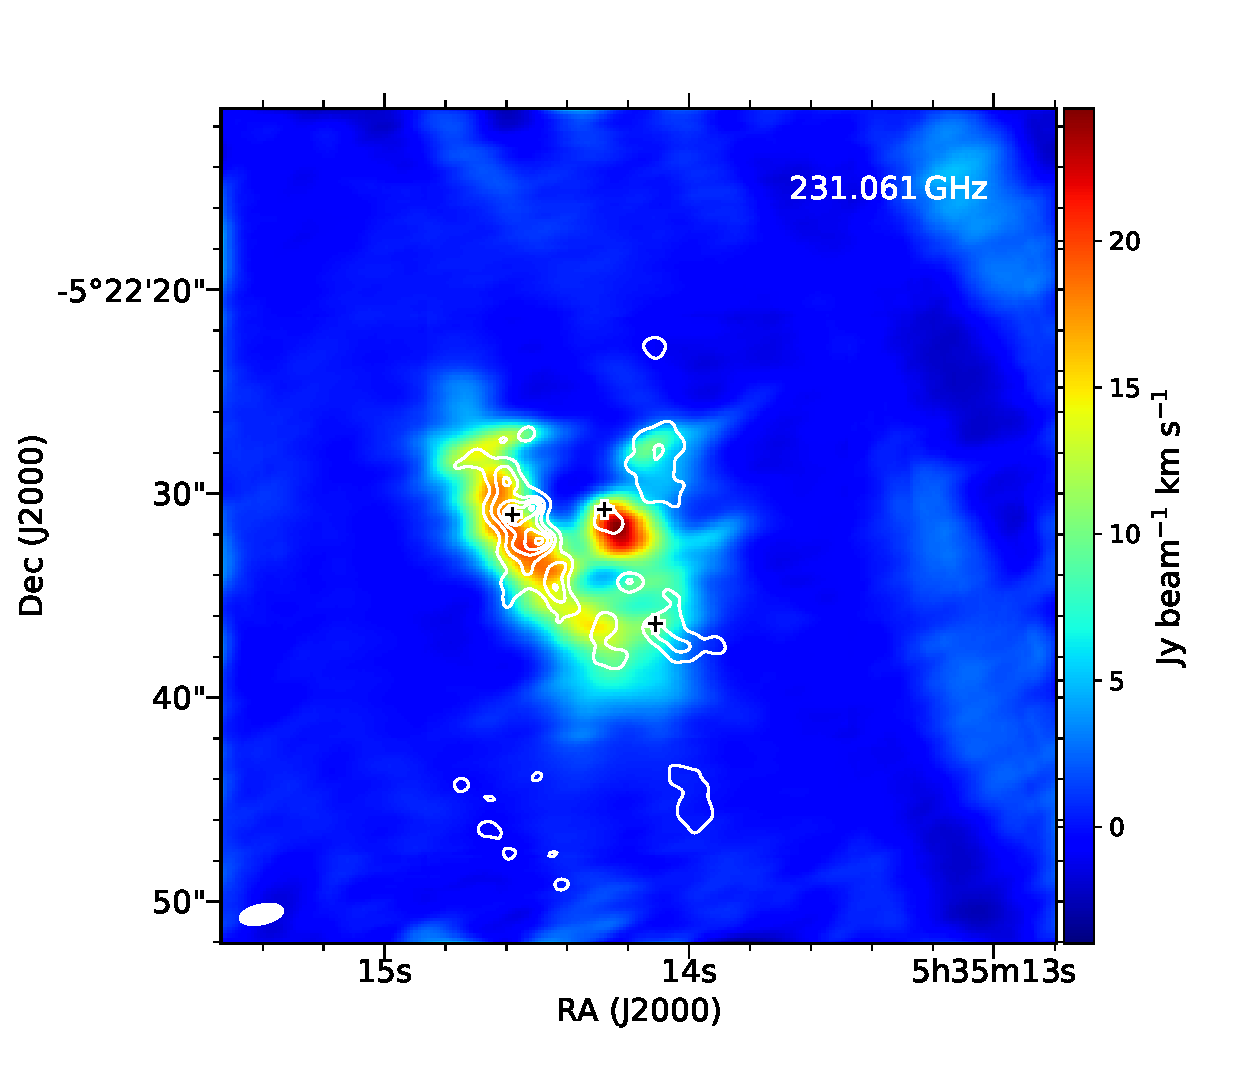
\includegraphics[width=0.98\textwidth]{OrionKL/mom0/231.061mom0_3-7.eps}
%\\(e) 左の図の説明
\end{center}
\end{minipage}
\begin{minipage}{0.48\textwidth}
\begin{center}
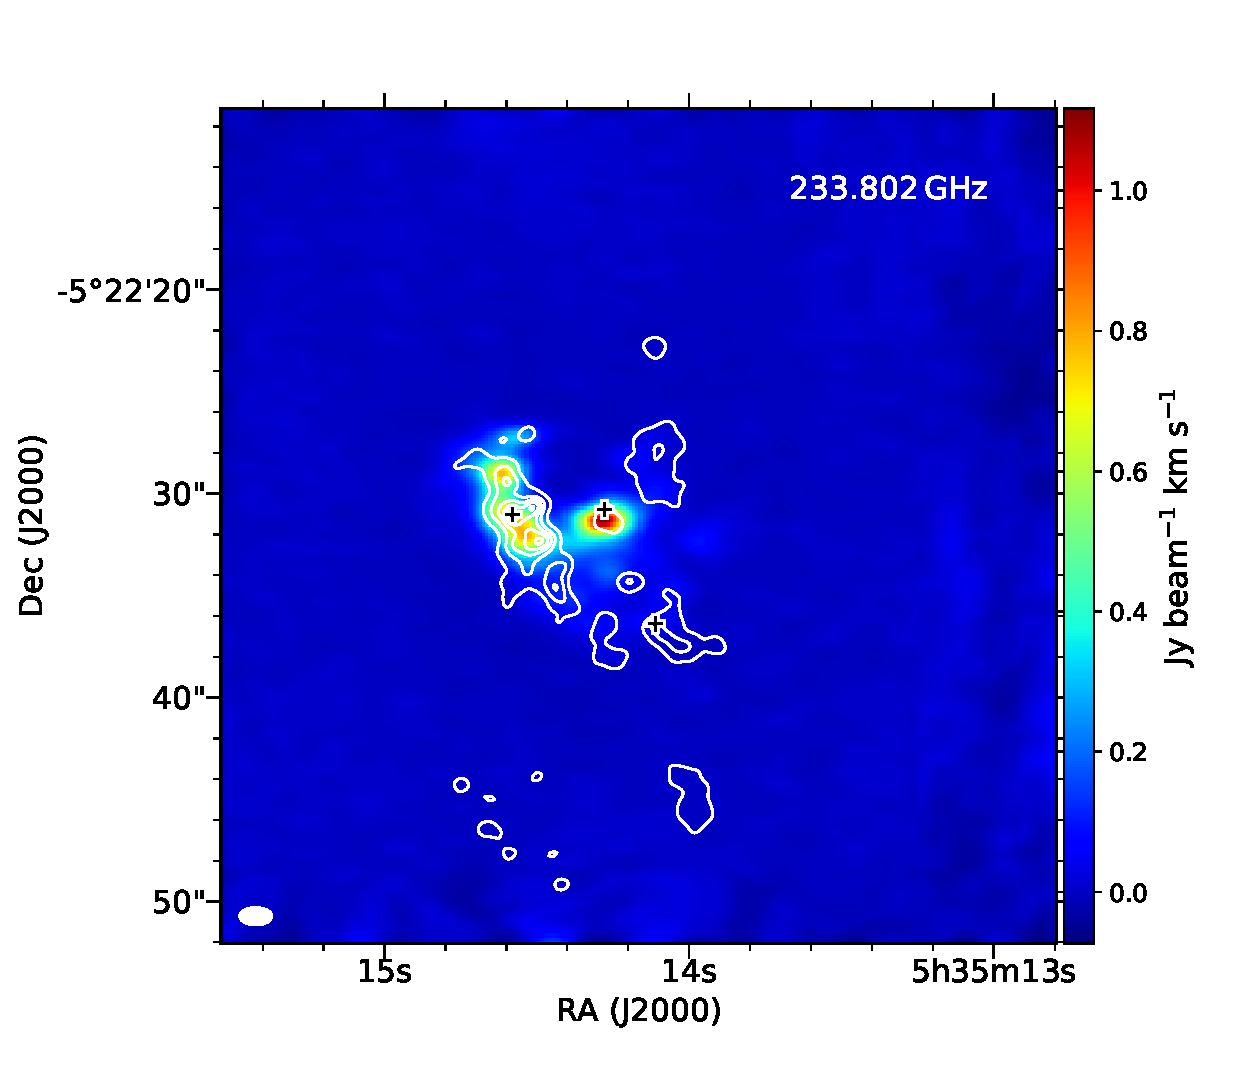
\includegraphics[width=0.98\textwidth]{OrionKL/mom0/233.802mom0_3-7.eps}
%\\(f) 右の図の説明
\end{center}
\end{minipage}
\end{center}
\end{minipage}
%%%% ここまで一組

%%%% ここから
\begin{minipage}{0.98\textwidth} 
\begin{center}
\begin{minipage}{0.48\textwidth}
\begin{center}
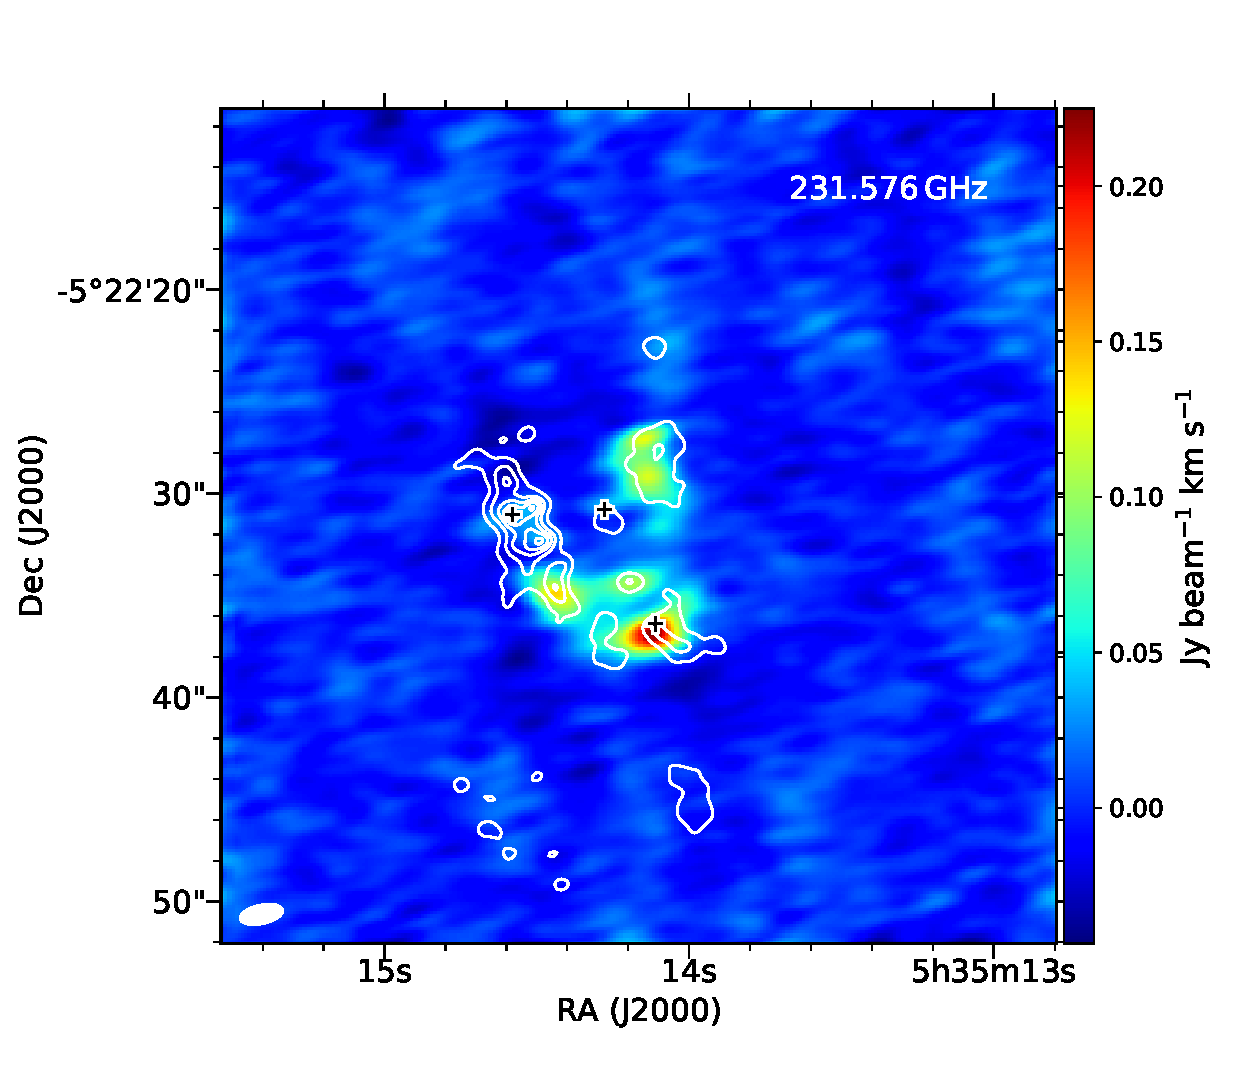
\includegraphics[width=0.98\textwidth]{OrionKL/mom0/231.576mom0_3-7.eps}
%\\(a) 左の図の説明
\end{center}
\end{minipage}
\begin{minipage}{0.48\textwidth}
\begin{center}
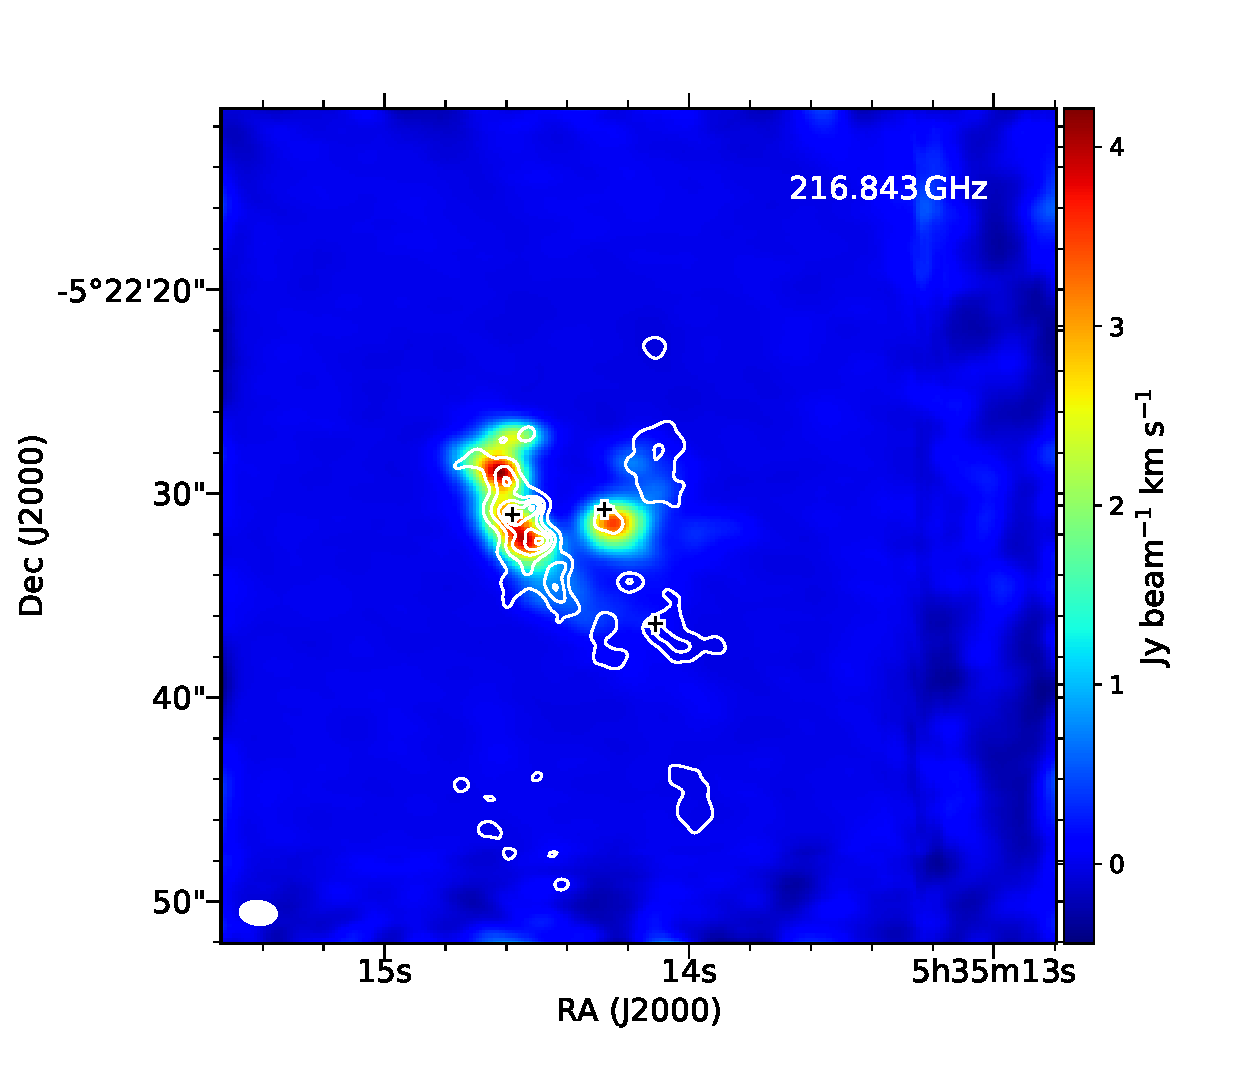
\includegraphics[width=0.98\textwidth]{OrionKL/mom0/216.843mom0_3-7.eps}
%\\(b) 右の図の説明
\end{center}
\end{minipage}
\end{center}
\end{minipage}
%%%% ここまで一組
\caption{(Continued)}
\end{center}
\end{figure}
%%%%%% ここまで

\begin{figure}[H] 
\begin{center}
%%%% ここから
\begin{minipage}{0.98\textwidth} 
\begin{center}
\begin{minipage}{0.48\textwidth}
\begin{center}
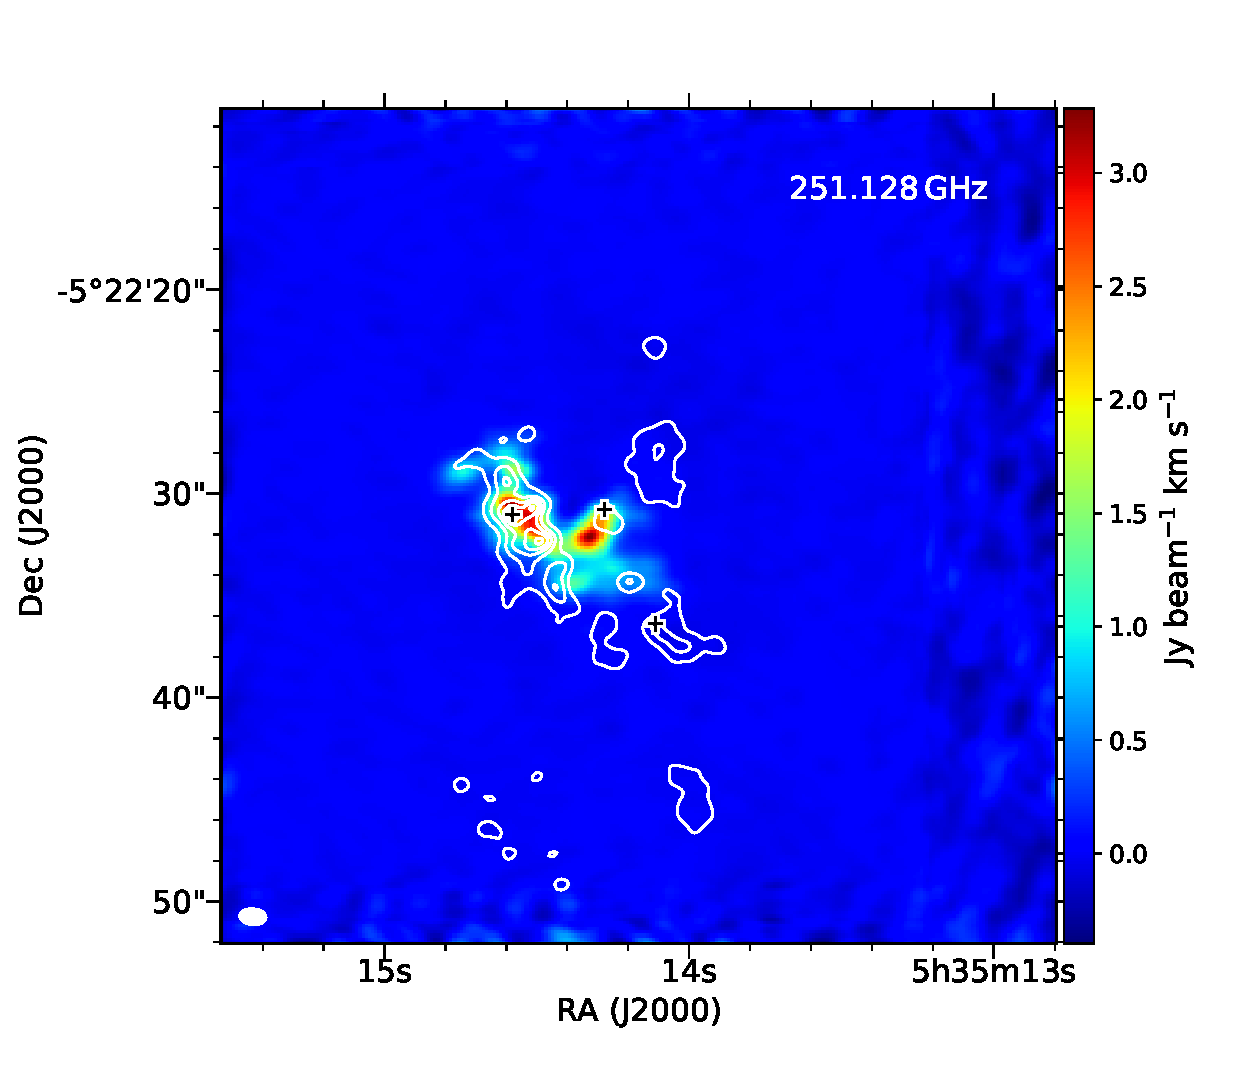
\includegraphics[width=0.98\textwidth]{OrionKL/mom0/251.128mom0_3-7.eps}
%\\(c) 左の図の説明
\end{center}
\end{minipage}
\begin{minipage}{0.48\textwidth}
\begin{center}
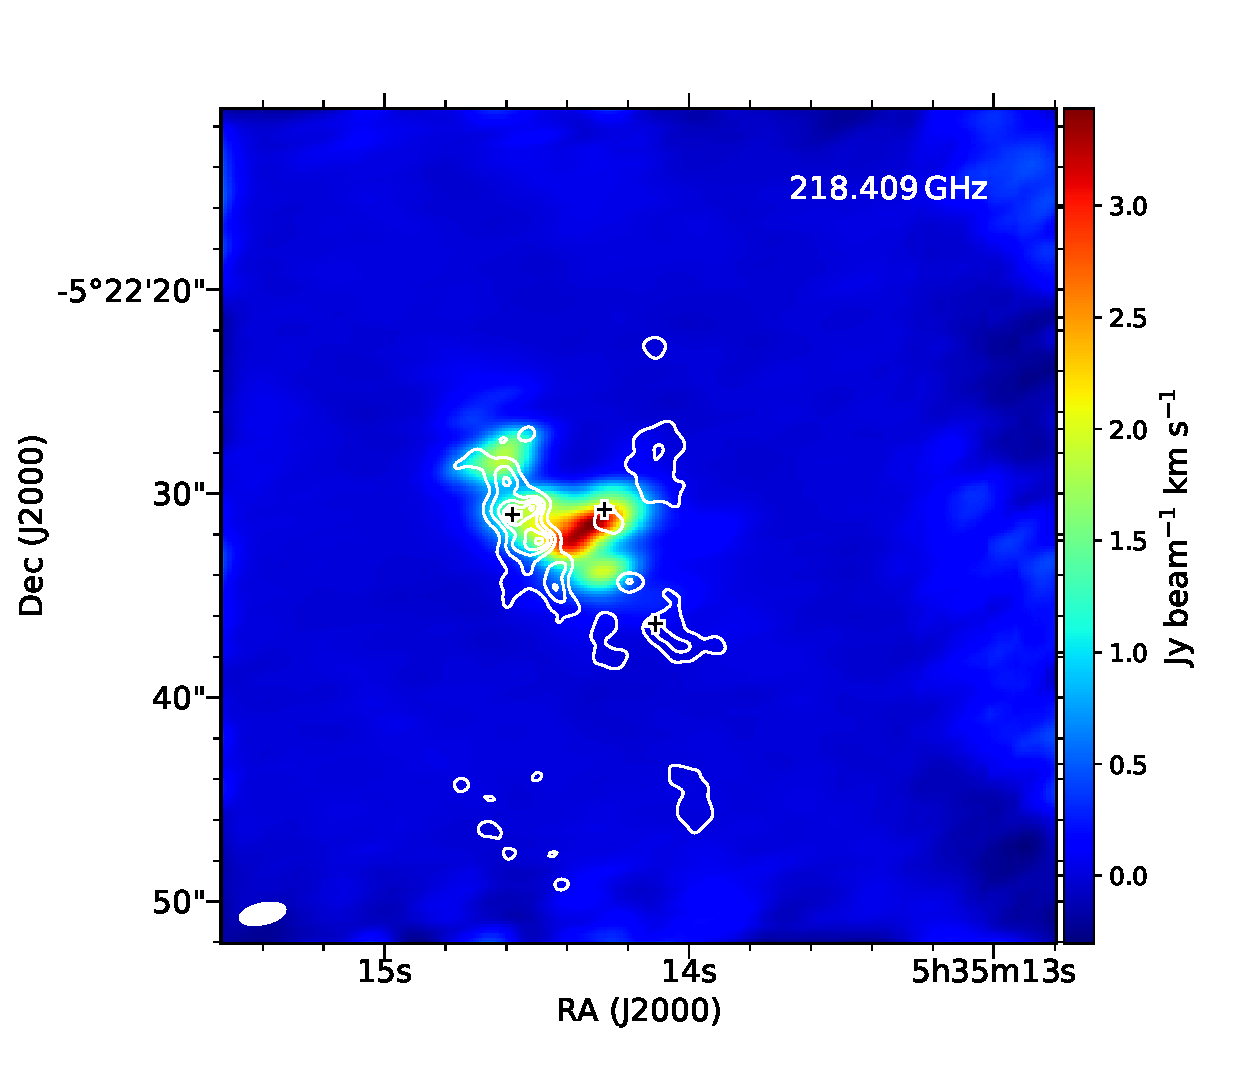
\includegraphics[width=0.98\textwidth]{OrionKL/mom0/218.409mom0_3-7.eps}
%\\(d) 右の図の説明
\end{center}
\end{minipage}
\end{center}
\end{minipage}

\begin{minipage}{0.98\textwidth} 
\begin{center}
\begin{minipage}{0.48\textwidth}
\begin{center}
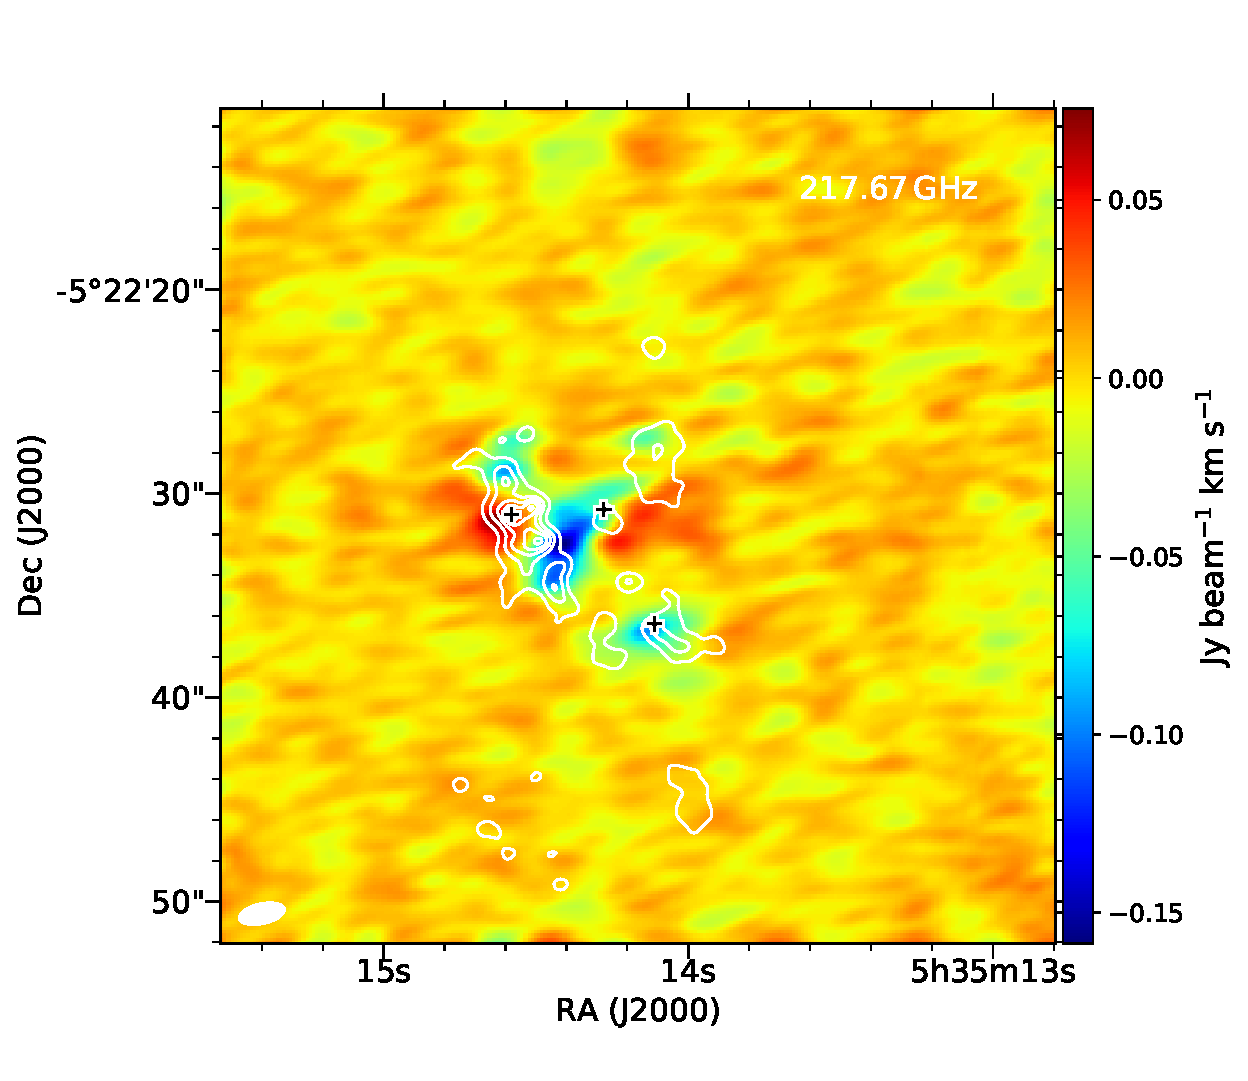
\includegraphics[width=0.98\textwidth]{OrionKL/mom0/217.67mom0_3-7.eps}
%\\(e) 左の図の説明
\end{center}
\end{minipage}
\begin{minipage}{0.48\textwidth}
\begin{center}
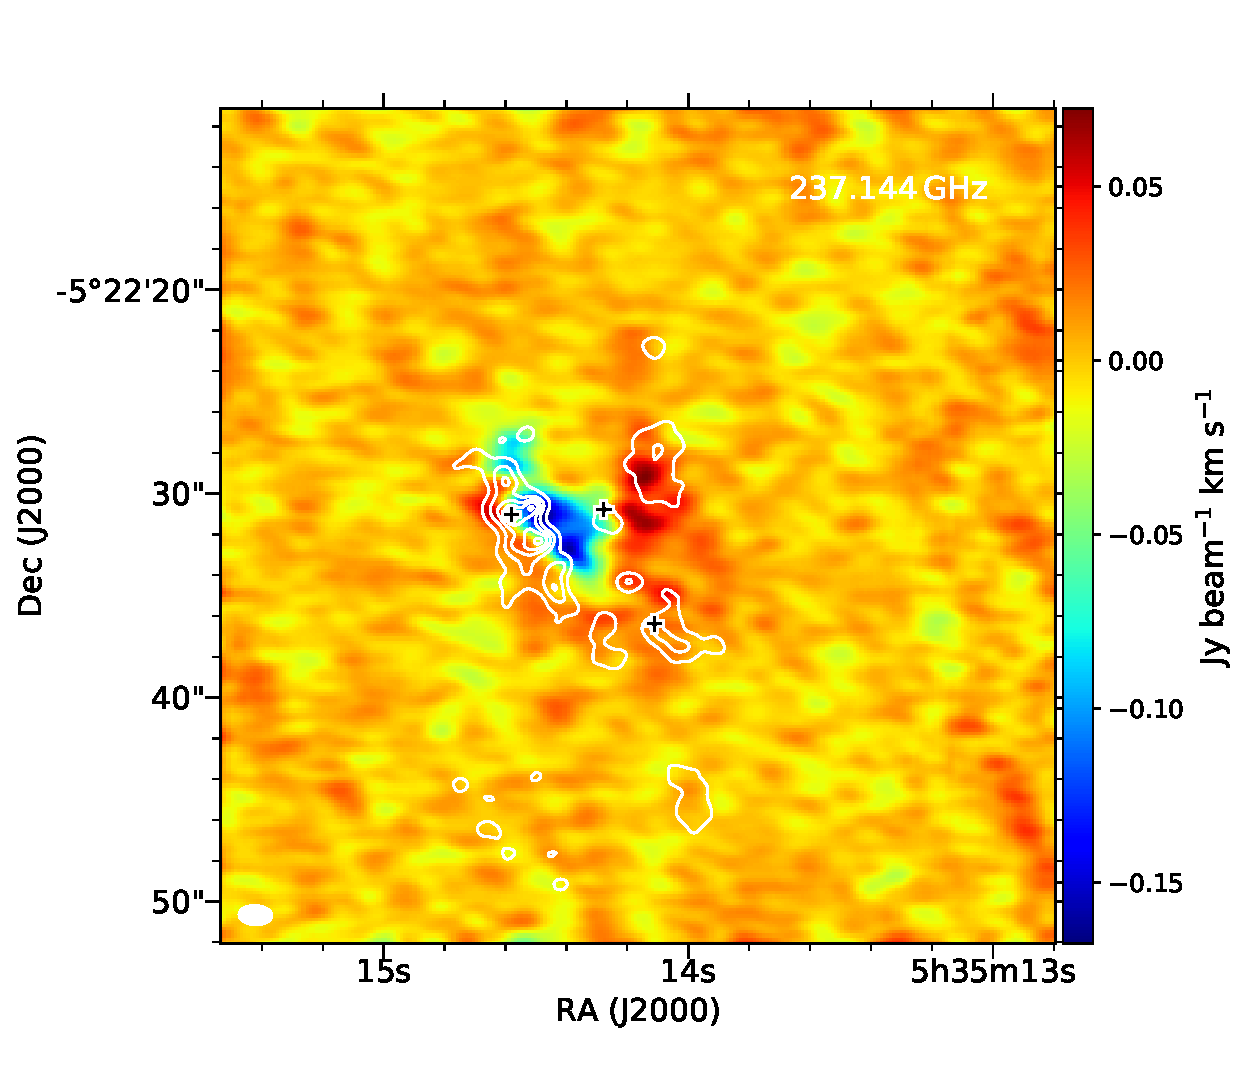
\includegraphics[width=0.98\textwidth]{OrionKL/mom0/237.144mom0_3-7.eps}
%\\(f) 右の図の説明
\end{center}
\end{minipage}
\end{center}
\end{minipage}
%%%% ここまで一組
\caption{(Continued)}
\end{center}
\end{figure}

\newpage

\section{Channel maps}

\begin{figure}[htbp]
  \centering
  \includegraphics[width=0.98\textwidth]{OrionKL/chmap/222.846.eps}
  \caption{222.846 GHz}
  \label{ap_ch_1}
\end{figure}

\begin{figure}[htbp]
  \centering
  \includegraphics[width=0.98\textwidth]{OrionKL/chmap/227.545.eps}
  \caption{227.545 GHz}
  \label{ap_ch_2}
\end{figure}

\begin{figure}[htbp]
  \centering
  \includegraphics[width=0.98\textwidth]{OrionKL/chmap/231.844.eps}
  \caption{231.844 GHz}
  \label{ap_ch_3}
\end{figure}

\begin{figure}[htbp]
  \centering
  \includegraphics[width=0.98\textwidth]{OrionKL/chmap/242.625.eps}
  \caption{242.625 GHz}
  \label{ap_ch_4}
\end{figure}

\begin{figure}[htbp]
  \centering
  \includegraphics[width=0.98\textwidth]{OrionKL/chmap/231.524.eps}
  \caption{231.524 GHz}
  \label{ap_ch_5}
\end{figure}

\begin{figure}[htbp]
  \centering
  \includegraphics[width=0.98\textwidth]{OrionKL/chmap/218.221.eps}
  \caption{218.221 GHz}
  \label{ap_ch_6}
\end{figure}

\begin{figure}[htbp]
  \centering
  \includegraphics[width=0.98\textwidth]{OrionKL/chmap/219.151.eps}
  \caption{219.151 GHz}
  \label{ap_ch_7}
\end{figure}

\begin{figure}[htbp]
  \centering
  \includegraphics[width=0.98\textwidth]{OrionKL/chmap/227.997.eps}
  \caption{227.997 GHz}
  \label{ap_ch_8}
\end{figure}

\begin{figure}[htbp]
  \centering
  \includegraphics[width=0.98\textwidth]{OrionKL/chmap/231.061.eps}
  \caption{231.061 GHz}
  \label{ap_ch_9}
\end{figure}

\begin{figure}[htbp]
  \centering
  \includegraphics[width=0.98\textwidth]{OrionKL/chmap/233.802.eps}
  \caption{233.802 GHz}
  \label{ap_ch_11}
\end{figure}

\begin{figure}[htbp]
  \centering
  \includegraphics[width=0.98\textwidth]{OrionKL/chmap/231.576.eps}
  \caption{231.576 GHz}
  \label{ap_ch_12}
\end{figure}

\begin{figure}[htbp]
  \centering
  \includegraphics[width=0.98\textwidth]{OrionKL/chmap/216.843.eps}
  \caption{216.843 GHz}
  \label{ap_ch_13}
\end{figure}

\begin{figure}[htbp]
  \centering
  \includegraphics[width=0.98\textwidth]{OrionKL/chmap/251.128.eps}
  \caption{251.128 GHz}
  \label{ap_ch_14}
\end{figure}

\begin{figure}[htbp]
  \centering
  \includegraphics[width=0.98\textwidth]{OrionKL/chmap/218.409.eps}
  \caption{218.409 GHz}
  \label{ap_ch_15}
\end{figure}

\begin{figure}[htbp]
  \centering
  \includegraphics[width=0.98\textwidth]{OrionKL/chmap/217.67.eps}
  \caption{217.670 GHz}
  \label{ap_ch_16}
\end{figure}

\begin{figure}[htbp]
  \centering
  \includegraphics[width=0.98\textwidth]{OrionKL/chmap/237.144.eps}
  \caption{237.144 GHz}
  \label{ap_ch_17}
\end{figure}